\section{Common privacy threats in software applications} \label{sec:common-privacy-concerns}
This section investigates how those privacy-related vulnerabilities identified in CWE and CVE (see Section \ref{sec:identifying-privacy-vul}) address common privacy threats in software applications. We first discuss a taxonomy of common privacy threats that we have developed based on an explanatory study of the literature. We then report the threats that have not been covered by the existing privacy-related vulnerabilities in CWE/CVE.

\subsection{Explanatory study}

To identify common privacy threats in practice, we performed an explanatory study on the literature of the following three groups: existing privacy software engineering (SE) research, well-established data protection regulations and privacy frameworks, and additional reputable resources. The details of this process are described below.

\subsubsection{Privacy engineering research}
Privacy engineering has attracted an emerging area of research in SE \cite{Gurses2016}. Our study in this area followed a systematic literature review process proposed by \cite{Kitchenham2007a} to retrieve relevant papers and conduct a literature survey. This process consists of three phases: planning, papers selection and extracting \& reporting.% (see Figure \ref{fig:process-explanatory}). 
In the planning phase, we defined our study goal which is to identify privacy threats addressed in the privacy engineering research. Our research question is ``What are privacy threats caused by software developers and/or relevant parties that were addressed in privacy engineering research?''. To achieve the study goal, we developed a review protocol to determine the scope of our study. The protocol consists of four tasks: (i) determining a search keyword and time scope, (ii) selecting SE publication venues, (iii) determining exclusion and inclusion criteria, and (iv) determining a set of questions to identify the privacy threats in the papers. In the papers selection phase, we conducted a search process and applied inclusion and exclusion to the retrieved papers. Finally, we analysed and identified privacy threats in the selected papers and reported the results.

%\begin{figure}[h]
%	\centering
%	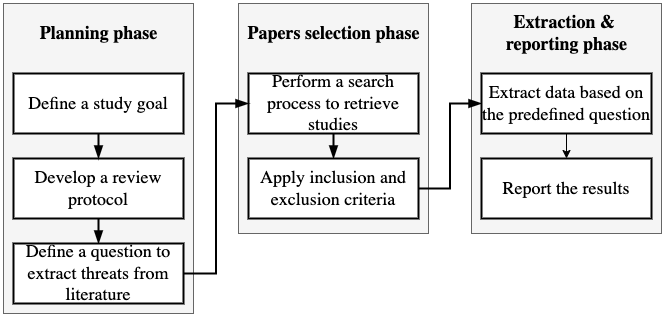
\includegraphics[width=1.0\linewidth]{figures/process-privacy-eng-research.png}
%	\caption{An overview process of privacy engineering research review.}
%	\label{fig:process-explanatory}
%\end{figure}

\paragraph{\textbf{Search keyword and time scope}}

We used a search keyword \emph{``privacy''} to search in title, abstract and keywords fields of papers in the selected publication venues. Only one search keyword was used as we already performed a search in the specific SE publication venues, thus we aimed to get all the papers that address privacy. In addition, the papers from these venues are peer-reviewed by experienced researchers in privacy and SE area, hence their significant contributions and quality are well received by the research community. We also determined to search for papers that were published in the past 20 years (2001 - 2020). This task was automatically done by the search functions in the academic databases (i.e. IEEE Xplore, ACM Digital Library, ScienceDirect, SpringerLink and Scopus). We have found 1,434 papers related to privacy during the period of 2001 to 2020 (see Figure \ref{fig:process-paper-selection}).

\begin{figure}[h]
	\centering
	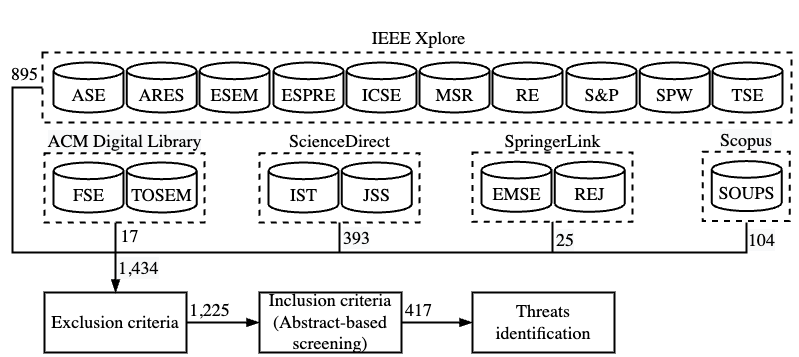
\includegraphics[width=1.0\linewidth]{figures/process-paper-selection.png}
	\caption{Number of papers included in each step.}
	\label{fig:process-paper-selection}
\end{figure}

\paragraph{\textbf{Software engineering publication venues}}

As privacy has also been widely addressed in other fields of study (e.g. law and social sciences), we scope down the search to get a reasonable number of papers in SE by selecting seventeen highly recognised SE publication venues consisting of 7 conferences, 6 journals, 2 symposiums and 2 workshops. These venues focus on various disciplines in SE, which make them proper candidates for representing privacy in multiple areas. Many of these venues were included in the existing papers that conducted systematic literature review in SE area (e.g. \cite{Ebrahimi2019, Perera2020a, Bertolino2018}). The full list of venues, along with the number of papers found in each, is included in the replication package. %Table \ref{tab:venues}.

\paragraph{\textbf{Exclusion and inclusion criteria}}

We manually performed an inclusion and exclusion task to ensure that the papers retrieved from the automated search process satisfy our study scope. We initially determined a set of inclusion and exclusion criteria to filter out the papers that are irrelevant to our goal. We exclude the papers that either contain insufficient, incomplete or irrelevant information (e.g. records that are journal/conference/workshop introduction, information from program chairs and summaries of keynotes), are duplicate \emph{OR} are secondary or tertiary studies (e.g. existing systematic literature review papers) and posters. For the inclusion criteria, we include the papers which their contribution is related to privacy \emph{AND} software development.


%The exclusion criteria (EC) are as follows:

%\begin{itemize}
%	\item \textbf{EC1:} Papers that contain insufficient, incomplete or irrelevant information (e.g. records that are journal/conference/workshop introduction, information from program chairs and summaries of keynotes). %As we automatically exported the records of studies from their databases, we found a number of records that contain journal/conference/workshop introduction, information from program chairs, guest editorials, summaries of keynotes and prefaces, which do not satisfy our study goal. Hence, those records are excluded from our study.
%	\item \textbf{EC2:} Papers that are duplicate. We consider from the title of the papers. If the papers have the exact same titles, other versions except the most recent version of those studies are excluded.
%	\item \textbf{EC3:} Papers that are secondary or tertiary studies (e.g. existing systematic literature review papers and systematic mapping studies) and posters are excluded.
%\end{itemize}

%The following inclusion criteria (IC) are applied in the screening step:
%
%\begin{itemize}
%	\item \textbf{IC1:} The primary contribution of the papers is related to privacy.
%	\item \textbf{IC2:} The research contribution of the papers is related to software development.
%\end{itemize}

After applying the EC, we excluded 209 out of 1,434 papers. 1,225 papers were passed to the next step. We then applied the IC to the abstracts of the papers. If the papers satisfy both IC, they are included in our study; otherwise they are excluded. Finally, 417 papers were included in our study\footnote{The bibliographic data of those papers are available in \cite{rep-pkg-privul}.}.

\begin{comment}
\begin{figure}[h]
	\centering
	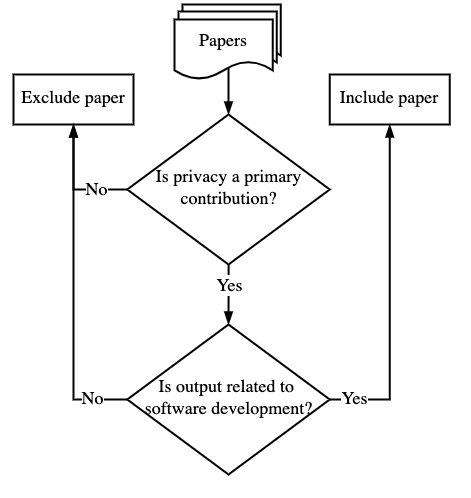
\includegraphics[width=1.0\linewidth]{figures/process-inclusion-criteria.png}
	\caption{Inclusion criteria.}
	\label{fig:process-inclusion-criteria}
\end{figure}
\end{comment}

\paragraph{\textbf{Privacy threats identification}}

To identify privacy threats, we examine the research studies reported in those papers, and shortlist the ones that focus specifically on privacy vulnerabilities and attacks from this list. The papers were analysed by asking the following questions:

\begin{itemize}[leftmargin=*]
	\item What is a cause of privacy-related problem in software that has been raised in the paper? This cause must involve personal data and is harmful to data subjects. %This question aims to list all the privacy threats addressed in the paper.
	\item Is the identified cause caused by software developers, data controllers/processors, organisations or external parties? This question helps us focus on the privacy threats that are not caused by users. There are papers that investigate user perceptions towards different privacy perspectives (e.g. user perceptions of online behavioural advertising/smart home devices and user confidence in using smartphones). We do not include the privacy threats that are caused by users in this study as it is out of our scope.
\end{itemize}

We manually examined the selected papers, and added privacy threats identified in the papers into a threat list. During the investigation, if we find a threat that is already included in our list, we annotate the paper with the existing threat and proceed to the next paper, otherwise we add a new threat into the list. Finally, we have found 179 papers that address privacy vulnerabilities and attacks in software development\footnote{See the file named \emph{``15-papers-by-threat-categories''} in the data folder in the replication package.}. From these studies, we have identified a range of privacy threats in various applications (e.g. mobile/web applications, mobile sensors, smart home devices, network communications and privacy policy compliance). These will be discussed in details in Section \ref{subsec:areas-of-concern}. The rest of the papers either address the threats caused by users or do not address privacy vulnerabilities or attacks in software systems.

%\begin{table*}[h]
	\caption{Selected software engineering publication venues.}
	\label{tab:venues}
	\begin{tabular}{p{8.5cm} p{1.25cm} p{1.5cm} p{1cm} p{1.25cm} p{1.25cm}}
		\toprule \textbf{Source title} & \textbf{Acronym} & \textbf{Type} & \textbf{Count} & \textbf{Included} & \textbf{Threats found} \\ \midrule
		ACM Transactions on Software Engineering and Methodology & TOSEM & Journal & 4 & 1 & 0\\
		Empirical Software Engineering & EMSE & Journal & 6 & 3 & 0\\
		IEEE Symposium on Security and Privacy & S\&P & Symposium & 330 & 64 & 9\\
		IEEE Symposium on Security and Privacy Workshops & SPW & Workshop & 134 & 49 & 5\\
		IEEE Transactions on Software Engineering & TSE & Journal & 22 & 7 & 1\\
		Information and Software Technology & IST & Journal & 16 & 5 & 0\\
		International Conference on Automated Software Engineering & ASE & Conference & 20 & 8 & 3\\
		International Conference on Availability, Reliability and Security & ARES & Conference & 186 & 113 & 93\\
		International Conference on Foundations of Software Engineering & FSE & Conference & 13 & 5 & 0\\
		International Conference on Mining Software Repositories & MSR & Conference & 8 & 2 & 0\\
		International Conference on Software Engineering & ICSE & Conference & 90 & 22 & 4\\
		International Requirements Engineering Conference & RE & Conference & 68 & 25 & 2\\
		International Symposium on Empirical Software Engineering and Measurement & ESEM & Conference & 5 & 1 & 0\\
		International Workshop on Evolving Security and Privacy Requirements Engineering & ESPRE & Workshop & 32 & 7 & 0\\
		Requirements Engineering & REJ & Journal & 19 & 10 & 2\\
		Symposium on Usable Privacy and Security & SOUPS & Symposium & 104 & 77 & 47 \\
		Systems and Software & JSS & Journal & 377 & 18 & 13 \\			
		\midrule
		\textbf{Sum} & & & \textbf{1,434} & \textbf{417} & \textbf{179} \\ \bottomrule
	\end{tabular}
\end{table*}


%\begin{table}[h]
%	\caption{Number of papers by threat subcategories.}
%	\label{tab:threats}
%	\begin{tabular}{p{6.25cm} p{1.25cm}}
%		\toprule \textbf{Threats} & \textbf{\#papers} \\ \midrule
%		Surveillance & 4 \\
%		Identification& 10 \\
%		Insecurity & 74 \\
%		Secondary use & 13 \\
%		Exclusion & 5 \\
%		Breach of confidentiality & 3 \\
%		Intrusions & 18 \\
%		Compliance & 31 \\
%		Multiple threats & 21 \\
%		Not a vulnerability/an attack & 238 \\	
%		\midrule
%		Total & 417 \\	
%		\bottomrule
%	\end{tabular}
%\end{table}


\subsubsection{Privacy regulations and frameworks}

We have studied 7 well-established data protection and privacy regulations and frameworks (i.e. GDPR \cite{OfficeJournaloftheEuropeanUnion;2016}, CCPA \cite{CCPA}, HIPAA \cite{HIPAA}, GLBA \cite{GLBA}, USPA \cite{US1974}, APA \cite{APA} and ISO/IEC 29100 \cite{ISO/IEC2011}). We have found that these regulations and frameworks focus mainly on the privacy threats related to the rights of individuals to control and be informed of their personal data processing. %They also raise a number of privacy threats related to individuals being informed about the processing (e.g. collection, use and transfer) of their personal data in software applications.

\subsubsection{Additional sources}
We have also included a range of relevant reputable organisations (e.g. OWASP and Norton) on this topic. These sources  (e.g. \cite{OWASP2020, Norton}) cover the recent trends of privacy risks and attacks. For example, OWASP identified 20 privacy risks in web applications \cite{OWASPsurvey} such as personal data leak, personal data stolen through common cyberattacks (e.g. cross-site scripting and broken session management). Norton also identified a number of social engineering cyberattacks that are privacy-related such as phishing and keystroke logging attacks \cite{Nortona}.

In the next section, we will discuss in details the common privacy threats that we have found in our explanatory study of the literature.

\subsection{A taxonomy of common privacy threats} \label{subsec:areas-of-concern}

We have built a taxonomy of common privacy threats upon the well-established privacy threats taxonomy described in \cite{Stallings2019}. The taxonomy was originally proposed by \cite{Solove2006a}. It covers privacy violations of individuals that are caused by physical activities (e.g. a newspaper reports the name of a rape victim, or a company sells its members' personal information despite promising not to do so). Later, \citeauthor{Stallings2019} adapted the concept from \cite{Solove2006a} to build the taxonomy of privacy threats for information systems. However, Stallings's taxonomy covers privacy threats in a generic and rather abstract level. Thus, we tailored this taxonomy and refined it into a more concrete version that addresses privacy threats in SE. The taxonomy consists of four categories of privacy threats: information collection, information processing, information dissemination and invasions (see Figure \ref{fig:AOC-vulnerabilities}). Each of these groups contains different subcategories covering relevant harmful privacy threats. The yellow boxes in Figure \ref{fig:AOC-vulnerabilities} represent the categories and subcategories included in the original taxonomy.

After identifying the privacy threats in the explanatory study, we classified those threats into two groups: vulnerabilities and compliance. Privacy vulnerabilities refer to technical issues, flaws or errors that lead to privacy exploits in software applications. Compliance addresses the privacy threats related to the individual rights and the governance of personal data. We then expanded the Stallings's taxonomy by mapping the privacy threats in the vulnerabilities group into their relevant subcategories in the original taxonomy (i.e. blue boxes in Figure \ref{fig:AOC-vulnerabilities}). However, the privacy threats in the compliance group have not been addressed in any groups in the original taxonomy. Thus, we propose the compliance group as an extension to the original taxonomy (see Figure \ref{fig:AOC-compliance}). This group is discussed in details in Section \ref{subsec:compliance}. The full taxonomy is available at \cite{rep-pkg-privul}.

In our taxonomy, we classified 24 privacy vulnerabilities into 7 subcategories. In the classification process, we mapped a privacy threat into the most relevant subcategory based on the description of each subcategory explained in \cite{Stallings2019}. The categories, subcategories and their relevant privacy threats are described below. We also provide several examples of sources where the privacy threats were raised or discussed in each category\footnote{See the file named \emph{``4-RQ2-explanatory-study-papers''} in the data folder in the replication package for the full list of papers with their associated privacy threats.}.

\begin{figure*}
	\centering
	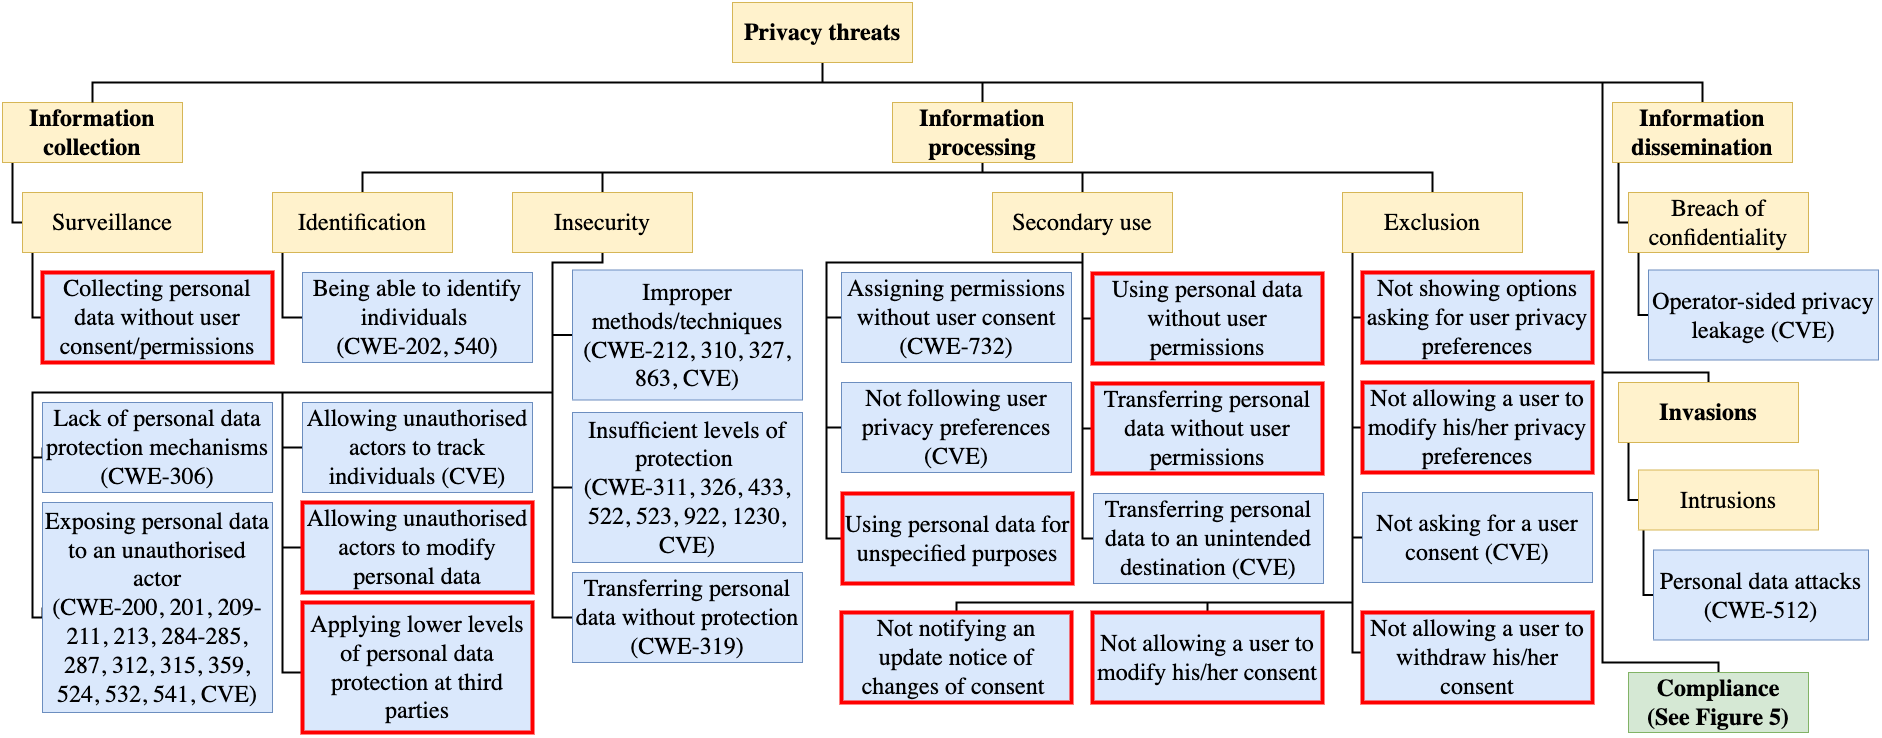
\includegraphics[width=1.0\linewidth]{figures/taxonomy.png}
	\caption{Common privacy vulnerabilities in software applications}
	\label{fig:AOC-vulnerabilities}
\end{figure*}


\subsubsection{\textbf{Information collection}} (Sources: \cite{De2016, Lebeck2018, Hasan2020, OfficeJournaloftheEuropeanUnion;2016, ISO/IEC2011, OWASPsurvey}) This category concerns privacy threats that occur when collecting personal data from individuals. The \emph{surveillance} subgroup covers vulnerabilities existing in the way software collects personal data such as watching individuals through cameras or CCTVs, listening to individuals, or recording individuals' activities. The privacy threat related to this subgroup occurs when personal data is collected without consent or permissions from individuals (e.g. via mobile sensors).

\subsubsection{\textbf{Information processing}} (Sources: \cite{Deng2011, Fisk2015, Figueiredo2017, Venkatadri2018, Some2019, Zhang2020a, HIPAA, GLBA}) This category covers vulnerabilities related to the use, storage, and manipulation of the collected personal data. It contains four subgroups: identification, insecurity, secondary use and exclusion. The \emph{identification} subcategory addresses a privacy threat that aggregates personal data from various sources and uses it to identify individuals.

The vulnerabilities in \emph{insecurity} subcategory are caused by improper protection and handling of personal data. There are multiple forms of this vulnerability type such as lacking mechanisms to protect personal data, allowing unauthorised actors to access or modify personal data, track individual users and transferring personal data without protection. Personal data is sometimes required to be processed at third parties. This poses a privacy vulnerability since the third parties may apply weaker level personal data protection than the source does. In addition, this subcategory refers to the vulnerabilities where mechanisms to protect personal data are in place but they are not appropriate. Different types of personal data require different methods/techniques and levels of protection. Thus, appropriate protection mechanisms should be used to protect personal data against potential risks. This vulnerability type is often refined into improper techniques/methods and insufficient levels of protection (e.g. weak encryption).

The \emph{secondary use} subcategory refers to the use of personal data for other purposes without consent or not following user privacy preferences. Personal data used or transferred without user permissions, or to an unintended destination is a privacy vulnerability. The personal data used without following user privacy preferences can also cause a privacy vulnerability\footnote{For example, CVE-2005-2512 reports a vulnerability which could result in a privacy leak in mail.app in Mac OS 10.4.2 and earlier in which remote images are loaded against the user's preferences when an HTML message is printed or forwarded.}.

The \emph{exclusion} subcategory refers to the failure to provide individuals with notice and input for managing their personal data. These vulnerabilities relate to consent which allows the users to express their agreement on the use of their personal data in software applications. We note that consent handling may seem to be a part of compliance, however this subcategory focuses on the malfunctions that cause vulnerabilities in consent handling. User consent is required when the processing of personal data is not required by laws. Users should also be notified when the conditions on the consent are changed. In addition, users should be allowed to modify or withdraw their consent. One example of this privacy vulnerability is in mobile applications where users allow a specific permission to an app, however the permission is overridden in other apps without their consent \cite{Calciati, Zhang2020a}. Apart from user consent, user privacy preferences are also important. Privacy preferences enable users to personalise how they prefer their personal data to be managed. This privacy vulnerability type can be in two forms: privacy preferences not provided to the users, and users not be able to modify their privacy preferences.

\subsubsection{\textbf{Information dissemination}} (Sources: \cite{Calciati, Jana2013, Lucia2012, Zhang2020a, OWASPsurvey}) This category refers to the privacy threats that lead to the disclosure of personal data to public. The \emph{breach of confidentiality} subcategory covers the vulnerabilities that cause personal data leakage by those who are responsible for personal data processing (e.g. software developers, data processors and third parties).

\subsubsection{\textbf{Invasions}} (Sources: \cite{Deng2011, Reinheimer2020, OWASPsurvey, Nortona}) This category addresses attacks that directly affect individuals. The \emph{intrusions} subcategory covers vulnerabilities exploited by common privacy attacks in software applications. There are typically four attacks: web applications, phishing, keystroke logging and smart home devices. %The attacks in web applications include, but not limited to, injection, broken authentication/authorisation/session management, security misconfigurations, cross-site request forgery (CSRF), insecure direct object reference (IDOR), using components with known vulnerabilities and invalidated redirects and forwards. Phishing attacks can be used to steal personal data by sending malicious links to the users through software applications, text messages and emails. These links bring the users to fake pages or programs that ask for their confidential data. The users are not aware of these malicious activities and end up giving away their personal data that can identify themselves (e.g. address, personal identifiers and financial data) to the attackers. Keystroke logging allows the attackers to track and record the keys that users have input on their keyboards. The attackers can then capture and steal personal data entered by users. Smart home devices are also vulnerable to external attacks. The attackers can intercept smart home systems to gain access to personal data.


\subsubsection{\textbf{Compliance}} \label{subsec:compliance}

We used a bottom-up approach to construct a taxonomy for the compliance category. The privacy threats that address the same concerns are grouped into the same subcategory. We classify privacy compliance into the following three subcategories. The first is \emph{not complying with individual rights} (Sources: \cite{OfficeJournaloftheEuropeanUnion;2016, CCPA, HIPAA, GLBA, US1974, APA, ISO/IEC2011, Deng2011, Omoronyia2013a, Bhatia2018a, Yu2021, Mihaylov2016a, OWASPsurvey}). There are 15 individual rights identified in our study\footnote{See the file named \emph{``14-rights''} in the data folder in the replication package for the complete list of individual rights.}. %(see Table \ref{tab:rights}).

The second is \emph{not providing contact details of a responsible person} (Sources: \cite{OfficeJournaloftheEuropeanUnion;2016, ISO/IEC2011}). This subcategory covers cases where software applications do not provide the contact details of a responsible person or a representative who processes personal data. This is a privacy threat as the users do not know whom to be contacted regarding their personal data processing. The third is \emph{improper personal data breach response} (Sources: \cite{OfficeJournaloftheEuropeanUnion;2016, ISO/IEC2011, HIPAA, OWASPsurvey}). When a breach occurs, a responsible person must notify two key stakeholders: concerned individuals and a supervisory authority. The privacy threat is raised if the responsible person does not communicate the breach incident to the concerned users whose personal data is leaked to the public and the supervisory authority who monitors the personal data processing under the individual rights.

\begin{figure}[ht]
	\centering
	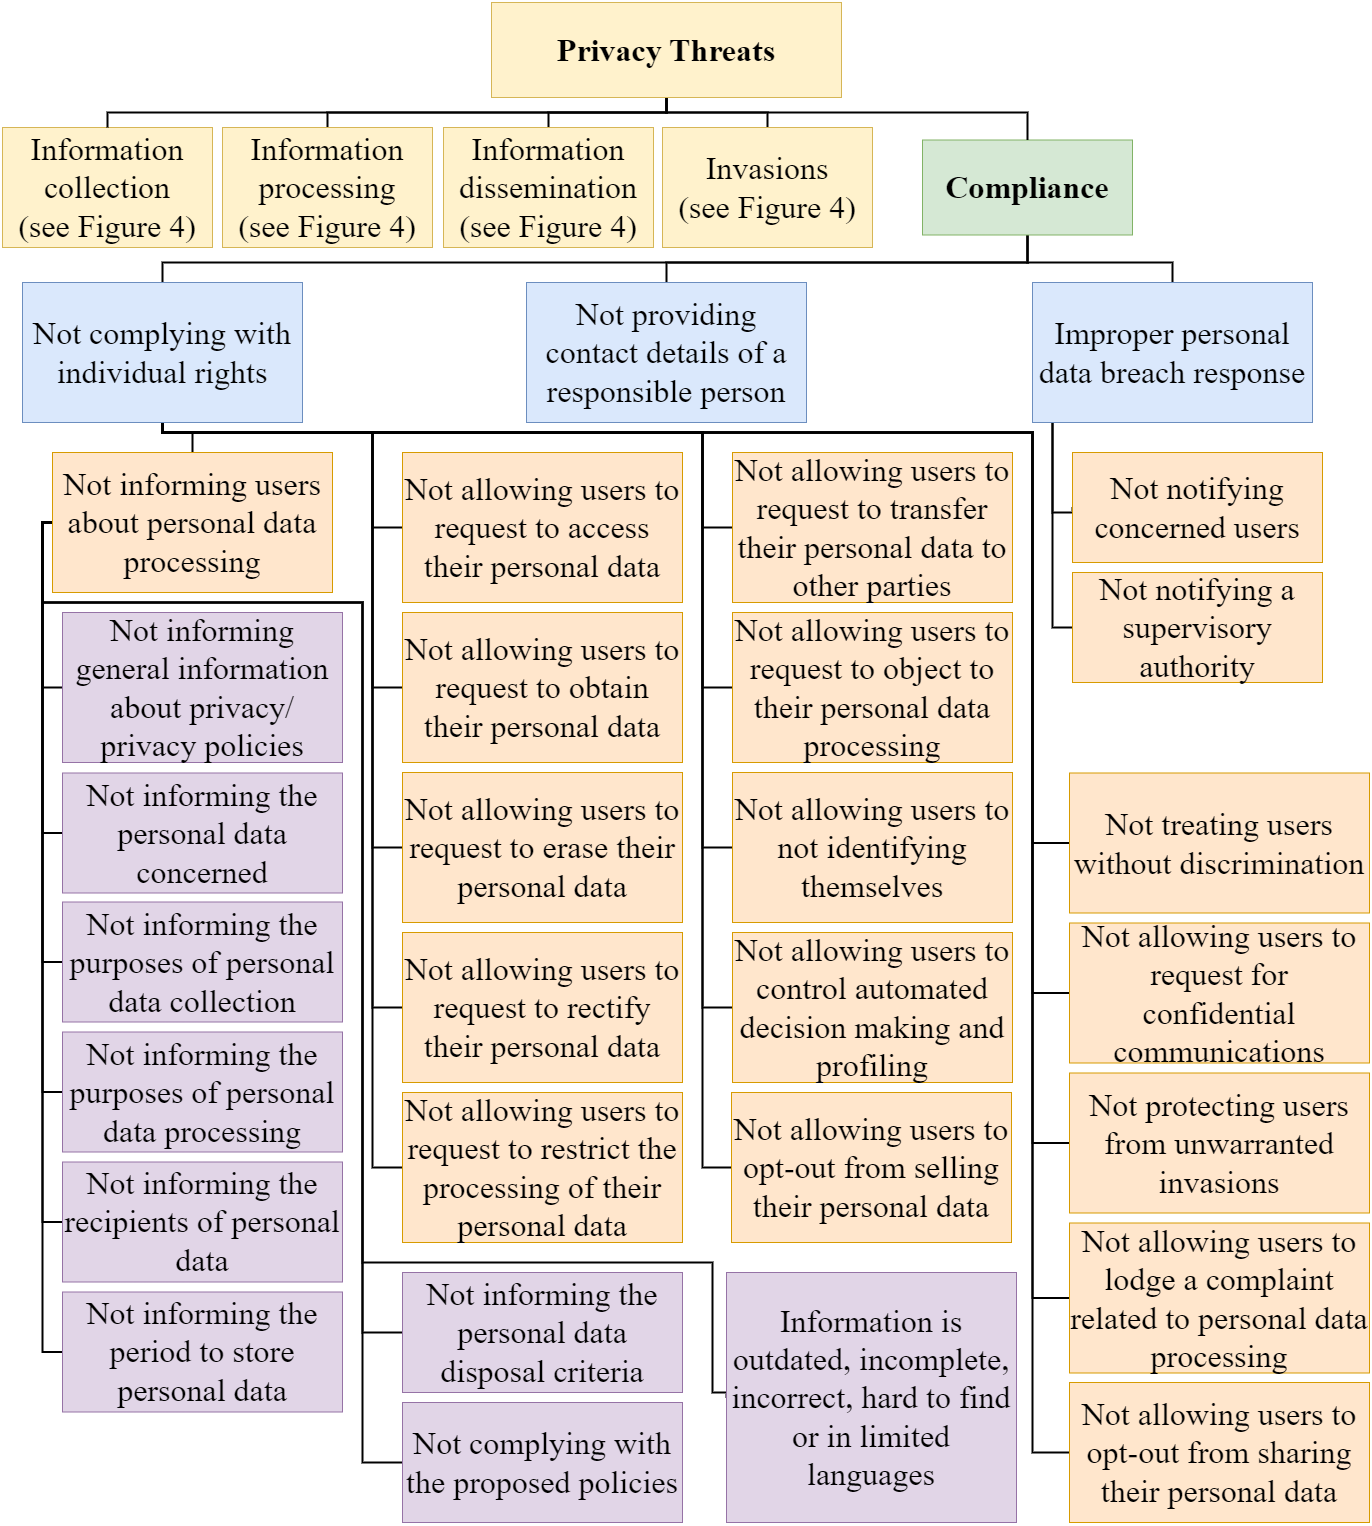
\includegraphics[width=\linewidth]{figures/taxonomy-compliance.png}
	\caption{Common privacy compliance in software applications}
	\label{fig:AOC-compliance}
\end{figure}

Our taxonomy covers the existing vulnerabilities occurred in a range of activities performed in software systems (e.g. personal data collection and processing). These privacy vulnerabilities have been raised in real world software applications and software development processes. The taxonomy was also developed based on an existing comprehensive privacy threats taxonomy, and validated with the common vulnerabilities reported in CWE and CVE.

\subsection{Privacy threats covered in CWE/CVE} \label{subsec:addressing-privacy-concerns}

The next step in our study was to investigate how 41 privacy vulnerabilities in CWE and 157 in CVE (see Section \ref{sec:identifying-privacy-vul}) address the taxonomy of common privacy threats in Section \ref{subsec:areas-of-concern}. This process consists of the following steps. The first two co-authors (hereafter referred to as the coders) \emph{independently} analysed each of the 41 privacy vulnerabilities in CWE, and classified it into the most relevant privacy threat in the taxonomy. Of the 157 privacy vulnerabilities in CVE, 112 were assigned to a specific CWE by the NVD. These 112 CVEs are automatically classified into the same privacy threat as their associated CWE. The remaining 45 CVEs, which were not assigned a specific CWE\footnote{NVD used two special placeholder names for these: NVD-CWE-noinfo and NVD-CWE-other.}, were manually classified by our coders. To facilitate the classification step, each coder was provided with a Google Sheet form pre-filled with the privacy vulnerabilities in CWE and CVE and the privacy threats in the taxonomy. The privacy threats were prepared as a drop down list. The coders then selected the vulnerability that is most relevant and best described those CWE and CVE in their view.

We have also employed the Inter-Rater Reliability (IRR) assessment and disagreement resolution processes to ensure the reliability of the classifications. The Cohen's Kappa coefficient is used to measure the inter-rater agreement as it is a perfect measure for a multi-class classification problem with two coders \cite{Hallgren}. Once the coders had completed the classifications, the inter-rater agreement was computed. The Kappa agreement values between the coders are 0.874 and 0.875 in CWE and CVE classifications respectively, which both achieve \emph{almost perfect agreement} level \cite{Viera2005}. A disagreement resolution was conducted to resolve some small classification conflicts (4 CWEs and 4 CVEs). The coders met, went through them together, discussed and reclassified those vulnerabilities. Thus, the final classification reached the maximum agreement between the coders.

\subsubsection{Results}

We have found that all the 41 CWEs and 157 CVEs together cover 13 vulnerabilities in the taxonomy. They are annotated with the corresponding CWEs and CVEs in Figure \ref{fig:AOC-vulnerabilities}. For brevity, we do not include the CVE numbers in Figure \ref{fig:AOC-vulnerabilities}, but they are provided in full in our replication package \cite{rep-pkg-privul}. Exposing personal data to an unauthorised actor, insufficient levels of protection, and personal data attacks are the top three most addressed vulnerabilities in both CWE and CVE. Personal data protection seems to attract a lot of attentions in CWE/CVE with more than half of the CWEs (56.1\%) and CVEs (59.87\%) vulnerabilities reported, most of which (36.59\% in CWEs and 50.32\% in CVEs) are related to exposing personal data to an unauthorised actor. There are 19.51\% in CWE and 15.92\% in CVE reporting vulnerabilities regarding personal data attacks.

There are four types of privacy vulnerabilities that are covered by both CWE and CVE: exposing personal data to an unauthorised actor, insufficient levels of personal data protection, improper methods/techniques for personal data protection, and personal data attacks. There are several types of privacy vulnerabilities that have been reported in CVE, but not in CWE, such as allowing unauthorised actors to track individuals, not following user privacy preferences, and not asking for user consent. 8.28\% of the CVEs refer to those types of privacy vulnerabilities, suggesting that those types of vulnerabilities need to be added into the CWE system.

A number of areas that are not covered by the existing privacy vulnerabilities in CWE and CVE are highlighted in red outline in Figure \ref{fig:AOC-vulnerabilities}. For example, exclusion involves a range of privacy vulnerabilities in failing to provide users with notice of user consent and input about their privacy preferences. User consent and privacy preferences are two essential mechanisms that enable users to control their personal data processing. These sources \cite{Antn2004, ISO/IEC2011, HIPAA} confirm that user privacy is vulnerable if users are not presented with options to specify or cannot modify their user privacy preferences. Similarly, user privacy may be  compromised if the users cannot modify or withdraw their consent, or are not notified about any changes of consent \cite{OfficeJournaloftheEuropeanUnion;2016, ISO/IEC2011, HIPAA, APA, OWASPsurvey}. However, none of them (except not asking for a user consent vulnerability) is covered in existing CVE.

Other areas that are not well covered in existing CWEs and CVEs are privacy vulnerabilities due to insecurity and secondary use. Processing personal data at a third party is a risk since they may apply weaker level personal data protection, particularly mobile \cite{Zhang2020a} and web applications \cite{OWASPsurvey}. There are cases that user privacy is violated when personal data is used for unspecified purposes or used or transferred without permissions (e.g. \cite{Hasan2020, De2016, Fisk2015, HIPAA, GLBA, US1974}). In addition, although allowing unauthorised actors to modify personal data and collecting personal data without user consent/permissions are serious threats, none of the existing privacy vulnerabilities in CWE and CVE covers this.

\begin{conclusion}
	\textbf{The existing privacy weaknesses and vulnerabilities reported in the CWE and CVE systems cover only 13 out of 24 common privacy vulnerabilities raised in research and practice.}
\end{conclusion} 